\chapter{Tracy-Widom Asymptotics}
In the last chapter we've determined explicitly the formula for $\mathbb{E}\left[ \frac{1}{(\zeta q^{X_n(t)}; q)_{\infty}} \right]$. This chapter will continue from this and perform asymptotic analysis for q-TASEP. The final result is that the fluctuation of the position of $X_N(t)$ will be following the GUE Tracy-Widom distribution. For simplicity, we assume through out the chapter that the jump rate parameters we are considering are $a_i = 1$ for all $i$, and that $q \in (0,1)$, $\theta > 0$ is fixed. 

\section{Tracy-Widom distribution}
We begin by providing a basic introduction to the GUE Tracy-Widom distribution. First the definition of the GUE Tracy-Widom distribution is quoted from \cite{phase2015} \textit{Definition 3 (1)}.

\begin{definition}
The GUE Tracy-Widom distribution is defined as $$F_{GUE}(r) = det(I-K_{Ai})_{L^2(r, \infty)},$$ where $K_{Ai}$ is the Airy kernel that has integral representations 
\begin{align*}
K_{Ai}(\eta, \eta') &= \frac{1}{(2 \pi i)^2} \int_{e^{-\frac{2 \pi i}{3}} \infty}^{e^{\frac{2 \pi i}{3}} \infty} dw \int_{e^{-\frac{\pi i}{3}} \infty}^{e^{\frac{\pi i}{3}} \infty} dz \frac{e^{z^3 / 3 - z \eta}}{e^{w^3 / 3 - w \eta'}} \frac{1}{z-w},
\end{align*}
where the contours for $z$ and $w$ do not intersect. 
\end{definition}
\begin{remark}
It's remarked that the Airy kernel defined above ie equivalent to $$K_{Ai}(\eta, \eta') = \int_{\mathbb{R}_+} d\lambda Ai(\eta+\lambda) Ai(\eta' + \lambda),$$
where $Ai(x)$ is the Airy function defined as
$$Ai(\eta) = \frac{1}{2 \pi i} \int_{C} \exp (\frac{z^3}{3} - z \eta) dz,$$ where $C$ is any contour starting at the point at infinity with argument $-\frac{\pi}{2}$ and ending at the point at infinity with argument $\frac{\pi}{2}$. Please refer to \cite{airy-kernel} for more details on the equality
\end{remark}

\section{Reformulation of Mellin-Barnes type kernel}
\label{sec:reformulation-kernel}
We provide the definitions of some parameters used in this section.

\begin{definition}
For fix $q \in (0,1)$ and $\theta > 0$, let the q-gamma function be defined as $$\Gamma_q(z) = (1-q)^{1-z} \frac{(q;q)_{\infty}}{(q^z;q)_{\infty}}$$ and the q-digamma function be defined as $$\Psi_q(z) = \frac{d}{d z} \log \Gamma_q(z) = -\log(1-q) + \log_q \sum_{n=1}^{\infty} \frac{q^{n+z}}{1 - q^{n+z}}.$$
Furthermore, we introduce the following parameters
\begin{equation}
\label{def:kappa}
\kappa = \kappa(q,\theta) = \frac{\Psi'_q(\theta)}{(\log q)^2 q^{\theta}} = \sum_{n=0}^{\infty} \frac{q^n}{(1-q^{n+\theta})^2};
\end{equation}
\begin{equation}
\label{def:f}
f = f(q,\theta) = \frac{\Psi'_q(\theta)}{(\log q)^2} - \frac{\Psi'_q(\theta)}{\log q} - \frac{\log(1-q)}{\log q};
\end{equation}
\begin{equation}
\label{def:chi}
\chi = \chi(q,\theta) = \frac{\Psi'_q(\theta) \log q - \Psi''_q(\theta)}{2}.
\end{equation}
\end{definition}

\begin{definition}
For any $c,x \in \mathbb{R}$, we define the following parameters
\begin{equation}
\label{def:tau}
\tau(N,c) = \kappa N + cq^{-\theta}N^{2/3}
\end{equation}
\begin{equation}
\label{def:macroscopic}
p(N,c) = (f-1)N + cN^{2/3} - c^2 \frac{(\log q)^3}{4 \chi} N^{1/3}
\end{equation}
The rescaled fluctuations, $\xi_N(c)$, of the $N^{th}$ particle at time $\tau(N,c)$ around $p(N,c)$ is defined to be 
\begin{equation}
\label{def:fluctuation}
\xi_N(c) = \frac{X_N(\tau(N,c)) - p(N,c)}{\chi^{1/3} (\log q)^{-1} N^{1/3}}. \\ \\
\end{equation}
\end{definition}
From \thmref{mbmb-application-to-qtasep}, we have that
\begin{equation}
\label{continuation-equation}
\mathbb{E} \left[ \frac{1}{(\zeta q^{X_N(t)+N}; q)_{\infty}} \right] = det(I+K_{\zeta}^{q-TASEP}),
\end{equation}
where $det(I+K_{\zeta}^{q-TASEP})$ is the Fredholm determinant of $K_{\zeta}^{q-TASEP}: L^2(C_{\mathbb{A}}) \rightarrow L^2(C_{\mathbb{A}})$ and the operator $K_{\zeta}^{q-TASEP}$ is defined in terms of its integral kernel
$$K_{\zeta}^{q-TASEP}(w,w') = \frac{1}{2 \pi i} \int_{C_{1,2,\dots}} \Gamma(-s) \Gamma(1+s) (-\zeta)^s \left(\frac{(q^s w; q)_{\infty}}{(w;q)_{\infty}}\right)^N \frac{e^{tw(q^s-1)}}{q^sw - w'} ds.$$
The main goal is this section is to perform some transformation for both sides of \eqref{continuation-equation}. For the right-hand side, we introduce the following change of variables 
\begin{equation}
\label{change-of-variables}
w = q^W, w' = q^{W'}, s+W = Z.
\end{equation}
Notice the Euler's Reflection formula that $\Gamma(-s) \Gamma(1+s) = \frac{\pi}{sin(-\pi s)}$, the kernel can be transformed to be 
\begin{align*}
& \quad \hat{K}_{\zeta}^{q-TASEP}(w,w') \\
& = \frac{q^W \log q}{2 \pi i} \int_{D^W_{R,d}} \frac{\pi}{sin(\pi (W-Z))} \frac{(-\zeta)^Z}{(-\zeta)^W} \frac{\exp(tq^Z+N\log(q^Z;q)_{\infty})}{\exp(tq^W+N\log(q^W;q)_{\infty})} \frac{dZ}{q^Z - q^{W'}}, \numberthis \label{eqn:rhs-mb}
\end{align*}
where $D^W_{R,d}$ is the contour $D_{R,d}$ shifted by $W$.\\

For the left-hand side, we first choose the parameter $\zeta$ in $\mathbb{E} \left[ \frac{1}{(\zeta q^{X_N(t)+N}; q)_{\infty}} \right]$ to be 
\begin{equation}
\label{zeta-choice}
\zeta = -q^{-fN - cN^{2/3} + \beta_x \frac{N^{1/3}}{\log q}} \in \mathbb{C} \setminus \mathbb{R}_+,
\end{equation}
\begin{equation*}
\beta_x = c^2 \frac{(\log q)^4}{4 \chi} - \chi^{1/3} x.
\end{equation*}
Notice that
\begin{align*}
-q^{ \frac{\chi^{1/3}}{\log q} N^{1/3} (\xi_N - x) } &= -q^{ \frac{\chi^{1/3}}{\log q} N^{1/3} (\frac{X_N(\tau(N,c)) - p(N,c)}{\chi^{1/3} (\log q)^{-1} N^{1/3}} - x) }\\
&= -q^{ X_N(\tau) - p(N,c) - \frac{\chi^{1/3}}{\log q} N^{1/3} x }\\
&= -q^{ X_N(\tau) - (f-1)N - cN^{2/3} + c^2 \frac{(\log q)^3}{4 \chi} N^{1/3}  - \frac{\chi^{1/3}}{\log q} N^{1/3} x} \\
&= \zeta q^{X_N(\tau) + N}.
\end{align*}
Therefore, we have the following equality that
\begin{equation}
\label{eqn:lhs-mb}
\mathbb{E} \left[ \frac{1}{(\zeta q^{X_N(\tau)+N}; q)_{\infty}} \right] = \mathbb{E} \left[ \frac{1}{( -q^{ \frac{\chi^{1/3}}{\log q} N^{1/3} (\xi_N - x) }; q )_{\infty}} \right]
\end{equation}
Combining \eqref{continuation-equation}, \eqref{eqn:rhs-mb} and \eqref{eqn:lhs-mb}, we have
\begin{equation}
\label{new-equality-mb-type}
\mathbb{E} \left[ \frac{1}{( -q^{ \frac{\chi^{1/3}}{\log q} N^{1/3} (\xi_N - x) }; q )_{\infty}} \right] = det(I+\hat{K}_{\zeta}^{q-TASEP})_{L^2(\hat{C}_{\mathbb{A}})},
\end{equation}
where 
\begin{align*}
& \quad \hat{K}_{\zeta}^{q-TASEP}(W,W') \\
& = \frac{q^W \log q}{2 \pi i} \int_{D^W_{R,d}} \frac{\pi}{sin(\pi (W-Z))} \frac{(-\zeta)^Z}{(-\zeta)^W} \frac{\exp(tq^Z+N\log(q^Z;q)_{\infty})}{\exp(tq^W+N\log(q^W;q)_{\infty})} \frac{dZ}{q^Z - q^{W'}}, \numberthis \label{transformed-kernel}
\end{align*}
where $\zeta$ is chosen as \eqref{zeta-choice}, given that both sides converge absolutely.

\section{Integration Contours}
\label{sec:integration-contours}
In this section, we give some concrete contours of $C_{\mathbb{A}}$ and $D_{R,d}$ that will ensure the convergence of the Fredholm determinants given in \eqref{continuation-equation}. We choose these contours also to facilitate our analysis later. We begin by defining some of the contours and then justify the convergence. 

\begin{figure}
	\centering
	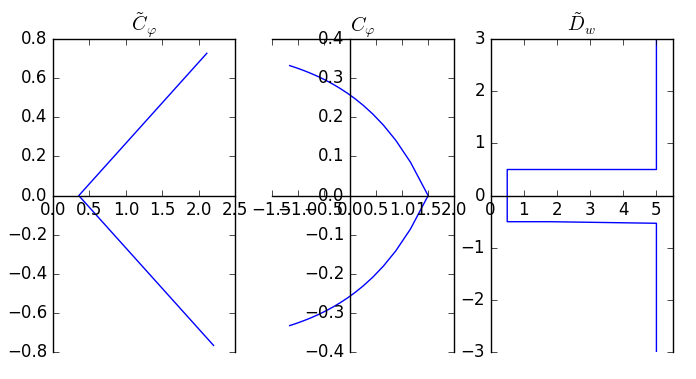
\includegraphics[width=\textwidth]{contour-cphi}
	\caption[The contours $\tilde{C}_{\varphi}$(left), $C_{\varphi}$(right) and $\tilde{D}_{w}$]
	{An illustration of the contours $\tilde{C}_{\varphi}$(left), $C_{\varphi}$(middle) for the parameter $q = 0.5$ and $\theta = 1.5$ and $\tilde{D}_{R,d}$(right) for the parameter $R = 5, d = 0.5$}
	\label{fig:cphi-contour}
\end{figure}

\begin{definition}
\label{contours-definition}
\begin{enumerate}
\item[(1)] Fix $q \in (0,1)$ and $\theta > 0$. For arbitrary but fix $\varphi \in (0, \pi / 4]$, we define the contour $\tilde{C}_{\varphi}$ to be $$\tilde{C}_{\varphi} = \{q^{\theta} + e^{i\varphi sgn(y)} |y|: y \in \mathbb{R}\}.$$ 
\item[(2)] Let $C_{\varphi}$ be the image of $\tilde{C}_{\varphi}$ under the mapping of $x \rightarrow \log_q(x)$. That is, $$C_{\varphi} = \{\log_q (q^{\theta} + e^{i\varphi sgn(y)} |y|) : y \in \mathbb{R}\}.$$
\item[(3)] For every $w \in \tilde{C}_{\varphi}$, define the contour $\tilde{D}_{w}$ to be $D_{R,d}$ as given in \textit{Section \ref{transformation-to-fd}} that it goes by straight lines from $R - i\infty$ to $R - id$, to $1/2 - id$, to $1/2 + id$, to $R + id$, and lastly to $R+i\infty$, with $R, d>0$ chosen such that the following holds:
\begin{enumerate}
\item[(a)] $arg(w(q^s-1)) \in (\pi / 2+b, 3\pi / 2 - b)$ for $b = \pi / 4 - \varphi / 2$;
\item[(b)] $q^sw$ stays to the left of $\tilde{C}_{\varphi}$ for every $s \in \tilde{D}_{w}$.
\end{enumerate}
\item[(4)] Lastly, for every $W \in C_{\varphi}$, we define the contour $D_W$ to be such that it is the contour $\tilde{D}_{q^W}$ shifted by $W$. If we let $R,d > 0$ be chosen for the contour $\tilde{D}_{q^W}$ such that the two conditions above are satisfied, then $D_W$ is defined by the straight lines going from $R+Re(W)-i \infty$ to $R+Re(W) + i(Im(W) - d)$, to $1/2+Re(W) + i(Im(W) - d)$, to $1/2 + Re(W) + i(Im(W) + d)$, to $R+Re(W) + i(Im(W) + d)$ and to $R+Re(W) + i \infty$.
\end{enumerate}

Please see \textit{Figure \ref{fig:cphi-contour}} for an illustration of the contours defined.
\end{definition}

\begin{proposition}
Fix $q \in (0,1)$, $\theta > 0$ and $\varphi \in (0, \pi / 4]$. Let $C_{\varphi}$ be defined as given in \textit{Definition \ref{contours-definition} (1)}. For every $W \in C_{\varphi}$ and the choice of $R, d$ such that the two conditions in \textit{Definition \ref{contours-definition} (3)} are satisfied with $w = q^W$. Then $$Re(W) + R > \theta.$$
\end{proposition}
\begin{remark}
An immediate result from the proposition is that there exists a $\sigma > 0$ such that $\theta + \sigma = R + Re(W)$. Moreover, the parameter $d > 0$ can be chosen to be so small such that $D_W$ and $C_{\varphi}$ do no intersect.
\end{remark}
\begin{proof}
This follows from \textit{Condition (b)} in \textit{Definition \ref{contours-definition} (3)}.
\end{proof}

We claim that with the choice of $C_{\mathbb{A}}$ to be $\tilde{C}_{\varphi}$ for any $\varphi \in (0, \pi / 4]$, and the choice of $C_{1, 2, \dots}$ to be $\tilde{D}_{w}$ for $w \in \tilde{C}_{\varphi}$, we have the convergence for the right-hand side of \textit{(\ref{continuation-equation})} as desired. To justify this, we only need to justify the three conditions in \textit{Theorem \ref{mbmb-application-to-qtasep}}, labeled as (1), (2), (3) respectively. For further details of the justification, please refer to \textit{\cite{asymptotics2013} Theorem (4.2)}.

Recall the change of variables \eqref{change-of-variables}, we have that the contour $\hat{C}_{\mathbb{A}}$ in \eqref{new-equality-mb-type} can then be chosen as $C_{\varphi}$ and that the contour $D_{R,d}^W$ for the integral kernel $\hat{K}_{\zeta}^{q-TASEP}(W,W')$ can be chosen as $D_W$. By further re-writing the kernel in the following form, we have the following result that for $x \in \mathbb{R}$, 
\begin{equation}
\label{new-equality-mb-type-2}
\mathbb{E} \left[ \frac{1}{( -q^{ \frac{\chi^{1/3}}{\log q} N^{1/3} (\xi_N - x) }; q )_{\infty}} \right] = det(I+K_x)_{L^2(C_{\varphi})},
\end{equation}
where 
\begin{align*}
& \quad K_x(W,W') \\
& = \frac{q^W \log q}{2 \pi i} \int_{D_W} \frac{dZ}{q^Z - q^{W'}} \frac{\pi}{sin(\pi (W-Z))} \frac{\exp(Nf_0(Z) + N^{2/3} f_1(Z) + N^{1/3} f_2(Z))}{\exp(Nf_0(W) + N^{2/3} f_1(W) + N^{1/3} f_2(W))},
\end{align*}
where
\begin{equation*}
f_0(Z) = -f (\log q) Z + \kappa q^Z + \log(q^Z; q)_{\infty}
\end{equation*}
\begin{equation*}
f_1(Z) = -c (\log q) Z + cq^{Z - \theta}
\end{equation*}
\begin{equation*}
f_2(Z) = \beta_x Z.
\end{equation*}

\begin{figure}
	\centering
	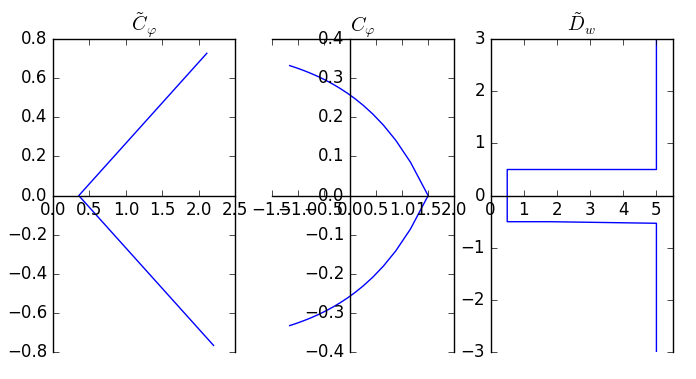
\includegraphics[width=\textwidth]{contour-cphi}
	\caption[Contour replacement of $D_W$]
	{An illustration of transformation of the contour $D_W$ mentioned in \textit{Remark \ref{circle-deformation}}}
	\label{fig:contour-dw-circle}
\end{figure}

\begin{remark}
\label{circle-deformation}
It's remarked that the contour $D_W$ in the definition of $K_x$ can be further replaced by the straight line from $R + Re(W) - i\infty$ to $R + Re(W) + i \infty$, where $R$ is the same as in the definition of $D_W$ and $d$ in the definition of $D_W$ is chose such that $D_W$ and $C_{\varphi}$ do no intersect, and some small circles surrounding the poles coming from the term $\frac{1}{sin(\pi (W - Z))}$, which are $W+1, W+2, \dots, W+k_W$ and $k_W$ denotes the total number of residues. The new contour will also be referred to as $D_W$. Please see \textit{Figure \ref{fig:contour-dw-circle}} for an illustration. 
\end{remark}

\section{Asymptotics of the Fredholm determinant}

In this section, we focus on the asymptotic behaviour of the Fredholm determinant in \eqref{new-equality-mb-type-2}. The main result is given in the following theorem.
\begin{theorem}
\label{asymptotic-theorem}
Let $x \in \mathbb{R}$ be fixed and choose $\zeta$ as in \textit{(\ref{zeta-choice})}. Then $$det(I+K_x)_{L^2(C_{\varphi})} \rightarrow F_{GUE}(x) \text{ as } N \rightarrow \infty,$$ where $F_{GUE}$ is the GUE Tracy-Widom distribution function. 
\end{theorem}

The intuition for the proof is that for $N$ large we show that the Fredholm determinants $det(I+K_x)_{L^2(C_{\varphi})}$ and $det(I-K_{Ai})_{L^2(x,\infty)}$ are arbitrarily close. To show how this can be achieved, we quote the following series of propositions from \cite{asymptotics2013} without proof and briefly explain the ideas behind. For more precise treatment, pleass refer to the original paper \cite{asymptotics2013} or \cite{phase2015}.

\begin{proposition} [\textit{\cite{asymptotics2013} Proposition (6.3)}]
\label{restriction-contour}
For any fixed $\delta > 0$ and $\epsilon > 0$ small enough, there is an $N_0$ such that $$\left| det(I+K_x)_{L^2(C_{\varphi})} - det(I+K_{x,\delta})_{L^2(C_{\varphi}^{\delta})} \right| < \epsilon$$ for all $N > N_0$ where
\begin{align*}
& \quad K_{x,\delta}(W,W') \\
& = \frac{q^W \log q}{2 \pi i} \int_{D_W^{\delta}} \frac{dZ}{q^Z - q^{W'}} \frac{\pi}{sin(\pi (W-Z))} \frac{\exp(Nf_0(Z) + N^{2/3} f_1(Z) + N^{1/3} f_2(Z))}{\exp(Nf_0(W) + N^{2/3} f_1(W) + N^{1/3} f_2(W))}
\end{align*}
and $C_{\varphi}^{\delta} = C_{\varphi} \cap \{w: |w - \theta| \le \epsilon \}$, $D_W^{\delta} = D_W \cap \{z: |z - \theta| \le \delta\}$.
\end{proposition}

This proposition essentially says that the asymptotically contribution to the Fredholm determinant outside any neighbourhood of $\theta$ can be ignored. Therefore, we only need to deal with the behavior of the Fredholm determinant around a small neighborhood of $\theta$. With this, the contour $C_{\varphi}$ and $D_{W}$ can be localized to a small neighborhood of $\theta$ (that is, $C_{\varphi}^{\delta}$ and $D_{W}^{\delta}$ respectively) without affecting the asymptotic behaviour of the determinant.

We then perform the following deformation of the contour $C_{\varphi}^{\delta}$ and $D_W^{\delta}$. Using Cauchy theorem, we are able to deform the contour $C_{\varphi}^{\delta}$ to $\{\theta + |y|e^{i(\pi - \tilde{\varphi}) sgn(y)}: y \in [-\delta, \delta]\}$ with some $\tilde{\varphi} \in (0, \pi / 2)$ chosen such that the two contours have the same endpoint. Similarly, we deform the straignt line $R+Re(W) + i \mathbb{R}$ in the contour $D_W^{\delta}$ to be $D_{\varphi}^{\delta} = \{\theta + |t| e^{i \varphi sgn(t)}: t \in [-\delta, \delta] \}$ if the $R$ in the definition of $D_W$ is chosen such that the two endpoints of the two contours coincide. 

After the above deformation, we introduce the following change of variables to $W, W'$ and $Z$: $$W = \theta + wN^{-1/3}, W' = \theta + w' N^{-1/3}, Z = \theta + zN^{-1/3}.$$ From the relationship, we get the corresponding contours for $w, w'$ and $z$ to be $C_{\varphi,\delta N^{1/3}}$ and $D_{\phi, \delta N^{1/3}}$, where
$$C_{\varphi,L} = \{|y|e^{i(\pi - \tilde{\varphi}) sgn(y)}: y \in [-L, L]\}, D_{\varphi, L} = \{|t| e^{i \varphi sgn(t)}: t \in [-L, L]\}$$ for $L \in (0, \infty].$ To be explicit, we have the following: $$det(I+K_{x, \delta})_{L^2(C_{\varphi}^{\delta})} = det(I +K_{x, \delta}^N )_{L^2(C_{\varphi, \delta N^{1/3}})},$$ where 
\begin{equation}
\label{rescaled-kernel}
K_{x, \delta}^N(w,w') = N^{-1/3} K_{x, \delta N^{1/3}} (\theta + wN^{-1/3}, \theta + w'N^{-1/3}).
\end{equation}

Moreover, from the definition of $f_0(Z), f_1(Z), f_2(Z)$, we have the following Taylor expansion of each of them around a neighborhood of $\theta$:
\begin{itemize}
\item $f_0(Z) = f_0(\theta) + \frac{\chi}{3} (Z - \theta)^3 + \mathcal{O}((Z - \theta)^4)$
\item $f_1(Z) = f_1(\theta) + \frac{c(\log q)^2}{2} (Z - \theta)^2 + \mathcal{O}((Z - \theta)^3)$
\item $f_2(Z) = f_2(\theta) + \beta_x (Z - \theta)$
\end{itemize}
Substituting these into (\ref{rescaled-kernel}), we can transform the kernel into the following explicit form as stated in the following proposition.

\begin{proposition} [\textit{\cite{asymptotics2013} Proposition (6.4)}]
Let $\varphi \in (0, \pi / 2)$ be sufficiently closed to $\pi / 2$ and let $\epsilon > 0$ be fixed. There is a small $\delta > 0$ and an $N_0$ such that for any $N > N_0$, $$|det(I +K_{x, \delta}^N )_{L^2(C_{\varphi, \delta N^{1/3}})} - det(I + K'_{x, \delta N^{1/3}})_{L^2(C_{\varphi, \delta N^{1/3}})}| < \epsilon,$$ where $$K'_{x,\delta N^{1/3}}(w,w') = \frac{1}{2 \pi i} \int_{D_{\varphi, \delta N^{1/3}}} \frac{dz}{(z-w')(w-z)} \frac{e^{\chi z^3 / 3 + c (\log q)^2 z^2 / 2 + \beta_x z}}{e^{\chi w^3 / 3 + c (\log q)^2 w^2 / 2 + \beta_x w}}.$$
\end{proposition}

The reason why we can choose $\varphi$ that is originally in $(0, \pi / 4]$ to be close to $\pi / 2$ is because of the following proposition.
\begin{proposition} [\textit{\cite{asymptotics2013} Proposition (6.2)}]
For fixed $q \in (0,1), \theta > 0$ and $N$ large enough, the contour $C_{\varphi}$ with $\varphi \in (0, \pi / 4)$ for the kernel $K_x$ can be extended to any $\varphi \in (0, \pi / 2)$ without affecting the Fredholm determinant $det(I+K_x)_{L^2(C_{\varphi})}$.
\end{proposition}

The following proposition asserts that we can expand the bound on the contour $D_{\varphi, \delta N^{1/3}}$ to $D_{\varphi, \infty}$. Similar to \textit{Proposition \ref{restriction-contour} }, we are essentially saying that asymptotically the only part of the contour that contributes to the Fredholm determinant is the part around some neighborhood of $0$. It is made precise by the following:

\begin{proposition} [\textit{\cite{asymptotics2013} Proposition (6.5)}]
As $N \rightarrow \infty$, we have $$det(I+K'_{x, \delta N^{1/3}})_{L^2(C_{\varphi, \delta N^{1/3}})} \rightarrow det(I+K'_{x, \infty})_{L^2(C_{\varphi, \infty})}.$$
\end{proposition}

And lastly, the kernel $K'_{x, \infty}$ can be reformulated to the Airy kernel via the following proposition.
\begin{proposition} [\textit{\cite{asymptotics2013} Proposition (6.6)}]

$$det(I+K'_{x,\infty})_{L^2(C_{\varphi, \infty})} = det(I - K_{Ai, x})_{L^2(\mathbb{R}_+)}.$$
\end{proposition}

By the definition of the GUE Tracy-Widom distribution introduced at the beginning of the chapter, we therefore conclude \textit{Theorem \ref{asymptotic-theorem}}.

\section{Distribution of the rescaled fluctuation}
In the last section, we concluded with \textit{Theorem \ref{asymptotic-theorem}} that for $N$ large, $det(I+K_x)_{L^2(C_{\varphi})} \rightarrow F_{GUE}(x)$. Therefore, 
\begin{equation}
\label{finale-equality}
\mathbb{E} \left[ \frac{1}{( -q^{ \frac{\chi^{1/3}}{\log q} N^{1/3} (\xi_N - x) }; q )_{\infty}} \right] \rightarrow F_{GUE}(x) \text{ as } N \rightarrow \infty.
\end{equation}
Define $f_N(y) = (-q^{\frac{\chi^{1/3}}{\log q} N^{1/3} y};q)_{\infty}^{-1}.$ Then we have that $$\mathbb{E} \left[ \frac{1}{( -q^{ \frac{\chi^{1/3}}{\log q} N^{1/3} (\xi_N - x) }; q )_{\infty}} \right] = \mathbb{E} \left[ f_N(\xi_N - x) \right].$$ We observe the following facts about $f_N(y)$:
\begin{itemize}
\item $f_N(y)$ is a mapping from $\mathbb{R}$ to $[0,1]$.
\item For each $N$, $f_N(y)$ is strictly decreasing on $y$. This is because $\log q < 0$ for $q \in (0,1)$. Moreover, $\lim_{y \rightarrow \infty} f_N(y) = 1$ and $\lim_{y \rightarrow -\infty} f_N(y) = 0$.
\item For each $\delta > 0$, on $\mathbb{R} \setminus [-\delta, \delta]$, the sequence of functions $f_N$ converges uniformly to $\mathbbm{1}(y < 0)$.
\end{itemize}
The last observation follows from the fact that $\frac{1}{1+q^{\frac{\chi^{1/3}}{\log q} N^{1/3} y + k}}$ is uniformly close to $1$ if $y \in (\delta, \infty)$ and $0$ if $y \in (-\infty, -\delta)$.

To continue our discussion, we quote the following lemma from \textit{\cite{macdonald2014} Lemma 4.1.39 }. 
\begin{lemma}
\label{last-lemma}
Consider a sequence of functions $(f_n)_{n \ge 1}$ mapping $\mathbb{R} \rightarrow [0,1]$ such that for eaach $n$, $f_n(y)$ is strictly decreasing in $y$ with a limit of $1$ at $y = -\infty$ and $0$ at $y = \infty$, and for each $\delta > 0$, on $\mathbb{R} \setminus [-\delta, \delta]$, $f_n$ converges uniformly to $\mathbbm{1}(y < 0)$. Consider a sequence of random variables $X_n(t)$ such that for each $r \in \mathbb{R}$, $$\mathbb{E} [f_n(X_n - r)] \rightarrow p(r)$$ and assume that $p(r)$ is a continuous probability distribution function. Then $X_n$ converges weakly in distribution to a random variable $X$ which is distributed according to $\mathbb{P}(X < r) = p(r)$.
\end{lemma}

Combining the lemma above, the observations about $f_N(y)$ and (\ref{finale-equality}), we conclude the following theorem.
\begin{theorem}
Let $q \in (0,1)$ and $\theta > 0$ be fixed. For any $c, x \in \mathbb{R}$, we have that $$\lim_{N \rightarrow \infty} \mathbb{P}(\xi_N < x) = F_{GUE}(x),$$ where $$\xi_N = \frac{X_N(\tau(N,c)) - p(N,c)}{\chi^{1/3} (\log q)^{-1} N^{1/3}}.$$
\end{theorem}
\begin{proof}
The proof is by applying Lemma \ref{last-lemma} directly with the sequence of functions $f_N(y)$.
\end{proof}